\documentclass[10pt]{beamer}

\usetheme{Madrid}
\usecolortheme{default}

% Base packages
%\usepackage{helvet}
\usepackage{amsmath,amssymb,amsthm,mathtools,subcaption}
\usepackage{tikz,pgfplots,tabularx,booktabs}
\usetikzlibrary{arrows.meta, positioning, quotes}

\usepackage{listings}
\usepackage{xcolor}

%\usepackage[cache=false]{minted}
%\renewcommand{\theFancyVerbLine}{\sffamily\textcolor[rgb]{0.5,0.5,1.0}{\scriptsize\oldstylenums{\arabic{FancyVerbLine}}}}
%\definecolor{bg}{rgb}{.95,.95,.95}

% Font settings
\renewcommand{\familydefault}{\sfdefault}

% TikZ libraries
\usetikzlibrary{calc,positioning,backgrounds,decorations.pathreplacing}
\pgfplotsset{compat=1.14}

% Colors
\definecolor{deepblue}{RGB}{42,39,155}
\definecolor{lightpink}{RGB}{255,240,240}
\definecolor{lightgreen}{RGB}{240,255,240}
\definecolor{lightyellow}{RGB}{255,255,240}
\definecolor{codegray}{RGB}{245,245,245}
\definecolor{codegreen}{rgb}{0,0.6,0}
\definecolor{codepurple}{rgb}{0.58,0,0.82}

% Beamer settings
\setbeamercolor{title}{fg=white,bg=deepblue}
\setbeamercolor{frametitle}{fg=white,bg=deepblue}
\setbeamercolor{section in head/foot}{fg=white,bg=deepblue}

\setbeamertemplate{footline}[text line]{%
  \parbox{\linewidth}{\vspace*{-8pt}
    \hfill
   \insertframenumber~/ \inserttotalframenumber}}
\setbeamertemplate{navigation symbols}{}%[only frame symbol]

\definecolor{foo}{rgb}{.2,.2,.7}
\AtBeginSection[]{
  \begin{frame}
  \vfill
  \centering
  \begin{beamercolorbox}[sep=8pt,center,shadow=true,rounded=true]{section page}
    \usebeamerfont{title}%
    {\color{foo} \insertsectionhead}\par%
  \end{beamercolorbox}
  \vfill
  \end{frame}
}

% https://tex.stackexchange.com/questions/30423/bibliography-in-beamer
\setbeamertemplate{bibliography entry title}{}
\setbeamertemplate{bibliography entry location}{}
\setbeamertemplate{bibliography entry note}{}

\DeclareMathOperator\prb{\mathsf{P}}
\DeclareMathOperator\expc{\mathsf{E}}
\DeclareMathOperator\var{var}
\DeclareMathOperator\cov{cov}
\DeclareMathOperator\cor{corr}
\DeclareMathOperator*{\argmax}{\arg\!\max}
\DeclareMathOperator*{\argmin}{\arg\!\min}
\DeclareMathOperator\corr{corr}
\DeclareMathOperator\rk{rank}
\DeclareMathOperator\sgn{sgn}
\DeclareMathOperator{\tr}{tr}

% Blackboard bold
\renewcommand{\AA}{\mathbb A}
\newcommand{\CC}{\mathbb C}
\newcommand{\DD}{\mathbb D}
\newcommand{\EE}{\mathbb E}
\newcommand{\FF}{\mathbb F}
\newcommand{\HH}{\mathbb H}
\newcommand{\KK}{\mathbb K}
\newcommand{\NN}{\mathbb N}
\newcommand{\PP}{\mathbb P}
\newcommand{\QQ}{\mathbb Q}
\newcommand{\RR}{\mathbb R}
\newcommand{\UU}{\mathbb U}
\newcommand{\ZZ}{\mathbb Z}

\newcommand{\ie}{\;\Longrightarrow\;}
\newcommand{\ifff}{\;\Longleftrightarrow\;}
\newcommand{\ds}{\displaystyle}

\title{Introduction to Financial Models \\ Lecture 03: Voting Theory}
\author{}
\date{}

\begin{document}

\begin{frame}
\titlepage
\end{frame}

\subsection*{Outline}
\begin{frame}
  \tableofcontents
\end{frame}

\section{Introduction to Voting}

\begin{frame}{Voting for Group Decision-Making}
  \begin{itemize}[<+->]
    \item Voting: A method to aggregate information across a group
    %\item Key differences between voting systems and markets:
    %  \begin{itemize}
    %    \item Voting explicitly tries to reach a \emph{single decision} that speaks for the group
    %    \item Markets synthesize opinions indirectly through transactions
    %    \item Market choices are often numerical and can be averaged
    %    \item Voting choices often lack natural averaging methods (e.g., choosing between candidates)
    %  \end{itemize}
    \item Types of voting applications:
      \begin{itemize}
        \item AI: Recommendation systems, PageRank algorithms (search engines), algorithmic decision-making, multi-agent systems
        \item Economics: Mechanism design, market design, public choice theory
        \item Political science: Electoral systems (population choosing candidates), legislative procedures (passing bills)
        \item Law: Jury decision rules (determining verdicts), judicial panels
        \item Business: Committee decision-making, corporate governance
        \item Critics' rankings (best movies, albums, etc.); Prize committees (selecting award recipients)
      \end{itemize}
    \item Voting can reflect genuine preference differences or different interpretations of information
  \end{itemize}
\end{frame}

\section{Individual Preferences}

\begin{frame}{Individual Preferences}
  \begin{itemize}[<+->]
    \item Each voter has a preference relation over alternatives
    \item Notation: $X \succ_i Y$ means voter $i$ prefers $X$ to $Y$ 
    \item Two key assumptions about rational preferences:
      \begin{itemize}
        \item \textbf{Completeness}: For any two alternatives $X$ and $Y$, either $X \succ_i Y$ or $Y \succ_i X$ (no abstention or indifference)
        \item \textbf{Transitivity}: If $X \succ_i Y$ and $Y \succ_i Z$, then $X \succ_i Z$ (consistency across choices)
      \end{itemize}
    \item Non-transitive preferences can be problematic:
      \begin{itemize}
        \item Example: If Chocolate $\succ_i$ Vanilla $\succ_i$ Strawberry $\succ_i$ Chocolate
        \item No ``best'' choice exists - each flavor is defeated by another
        \item Leads to indecision or exploitation in sequential choices
      \end{itemize}
    \item If preferences are complete and transitive, they correspond to a ranked list
    \item Mathematically provable: Any complete and transitive preferences can be represented as a ranked list, and vice versa
  \end{itemize}
\end{frame}

\section{Voting Paradox}

\begin{frame}{Voting Paradox (Condorcet Paradox)}
  \begin{itemize}
    \item The Simplest Case: Three voters, three alternatives
      \begin{table}
        \center
        \begin{tabular}{cccc}
          \toprule
          \textbf{Voter} & \textbf{First preference} & \textbf{Second preference} & \textbf{Third preference} \\
          \midrule
          Voter 1 & A & B & C \\
          Voter 2 & B & C & A \\
          Voter 3 & C & A & B \\
          \bottomrule
        \end{tabular}
      \end{table}
    \item Each voter has rational (transitive) preferences
    \item Majority rule on pairs produces:
      \begin{itemize}
        \item A beats B (voters 1 and 3)
        \item B beats C (voters 1 and 2)
        \item C beats A (voters 2 and 3)
      \end{itemize}
    \item Result: Cyclic group preferences despite transitive individual preferences
    \item Paradox: Even with rational individuals, the group can be ``irrational''
    \item This creates fundamental problems for democratic decision-making
  \end{itemize}
\end{frame}

\begin{frame}{Voting Paradox in Social Contexts}
  \begin{itemize}
    \item A More Complicated Situation: Party preferences over spending priorities
      \begin{table}
        \center
        \begin{tabular}{llll}
          \toprule
          \textbf{Party} & \textbf{First preference} & \textbf{Second preference} & \textbf{Third preference} \\
          \midrule
          Left (3)   & education & health & security \\
          Center (4) & health & security & education \\
          Right (5)  & security & education & health \\
          \bottomrule
        \end{tabular}
      \end{table}
    \item Individual vs. Multi-criteria decision making:
      \begin{itemize}
        \item The paradox can arise even for a single individual deciding between options with multiple criteria
        \item Example: College choice based on ranking, class size, and scholarship money
      \end{itemize}
      \begin{table}
        \center
        \begin{tabular}{cccc}
          \toprule
          \textbf{College} & \textbf{National Ranking} & \textbf{Average Class Size} & \textbf{Scholarship Money} \\
          \midrule
          A & 4 & 40 & \$3000 \\
          B & 8 & 18 & \$1000 \\
          C & 12 & 24 & \$8000 \\
          \bottomrule
        \end{tabular}
      \end{table}
      \begin{itemize}
        \item When each option wins on different criteria, cycling can occur
      \end{itemize}
  \end{itemize}
\end{frame}

\section{Voting Systems: Majority Rule}

\begin{frame}{Voting Systems: Majority Rule}
  \begin{itemize}[<+->]
    \item For two alternatives: the alternative preferred by majority wins
      \begin{itemize}
        \item Natural, intuitive, and widely accepted
        \item Treats all voters equally
        \item Produces a complete, transitive ranking
      \end{itemize}
    \item For three or more alternatives:
      \begin{itemize}
        \item Create group preferences by majority vote on each pair (pairwise comparisons)
        \item Problem: Group preferences may not be transitive (Condorcet Paradox)
        \item Cannot simply produce a ranked list when cycles occur
      \end{itemize}
    \item Elimination tournaments based on majority rule:
      \begin{itemize}
        \item Structure comparisons as sequential eliminations
        \item Arrange alternatives in pairs for voting
        \item The winner advances to face the next alternative
        \item Continue until overall winner emerges
      \end{itemize}
    \item Key insight: The ordering of the pairs (the ``agenda'') affects the outcome
    \item Raises concerns about fairness and manipulation
  \end{itemize}
\end{frame}

\begin{frame}{Example of Strategic Agenda-Setting}
  \begin{itemize}[<+->]
    \item Individual rankings:
      \begin{itemize}
        \item Voter 1: $X$ $\succ$ $Y$ $\succ$ Z
        \item Voter 2: $Y$ $\succ$ $Z$ $\succ$ X
        \item Voter 3: $Z$ $\succ$ $X$ $\succ$ Y
      \end{itemize}
    \item Pairwise majority votes:
      \begin{itemize}
        \item $X$ beats $Y$ (voters 1 and 3)
        \item $Y$ beats $Z$ (voters 1 and 2)
        \item $Z$ beats $X$ (voters 2 and 3)
      \end{itemize}
    \item Agenda manipulation through different tournament structures:
      %\begin{figure}
      % \centering
      %  \begin{tikzpicture}[node distance=1.5cm]
      %    \node (X) {X};
      %    \node (Y) [right of=X] {Y};
      %    \node (w1) [above right of=X, xshift=0.5cm] {X wins};
      %    \node (Z) [right of=w1, xshift=1cm] {Z};
      %    \node (out) [above right of=w1, xshift=1cm] {Z wins overall};
      %    
      %    \draw[->] (X) -- (w1);
      %    \draw[->] (Y) -- (X);
      %    \draw[->] (w1) -- (out);
      %    \draw[->] (Z) -- (out);
      %  \end{tikzpicture}
      %\end{figure}
      \begin{itemize}
        \item Agenda 1: $X$ vs $Y$ first, then winner vs $Z$ $\ie$ $Z$ wins
        \item Agenda 2: $Y$ vs $Z$ first, then winner vs $X$ $\ie$ $X$ wins
        \item Agenda 3: $X$ vs $Z$ first, then winner vs $Y$ $\ie$ $Y$ wins
      \end{itemize}
    \item Power of agenda-setting: The person who controls the order of voting can determine the outcome
    \item Real-world impact: Parliamentary procedure, committee votes, and meeting agendas all involve this kind of strategic sequencing
  \end{itemize}
\end{frame}

\section{Voting Systems: Positional Voting}

\begin{frame}{Positional Voting Systems}
  \begin{itemize}[<+->]
    \item Direct approach: Assign weights based on position in each voter's ranking
    \item Borda Count: Named after Jean-Charles de Borda (1770)
      \begin{itemize}
        \item With $k$ alternatives: $k-1$ points for first place, $k-2$ for second, etc.
        \item Each alternative receives points based on its positions in all rankings
        \item Alternatives ranked by total points received
        \item Used in: Heisman Trophy, AP poll rankings, MLB MVP selection
      \end{itemize}
    \item Plurality voting:
      \begin{itemize}
        \item $1$ point for first place, $0$ for all others
        \item Special case of positional voting
        \item Used in: Most political elections, ``first past the post'' systems
      \end{itemize}
    \item Advantages:
      \begin{itemize}
        \item Always produces a complete, transitive ranking
        \item Considers all positions in rankings (Borda)
        \item Simple to implement and understand
      \end{itemize}
    \item Key problems:
      \begin{itemize}
        \item Results can be manipulated by strategic voting
        \item ``Irrelevant'' alternatives can change the outcome
        \item Vulnerable to strategic addition or removal of alternatives
      \end{itemize}
  \end{itemize}
\end{frame}

\begin{frame}{Example of Borda Count}
  \begin{itemize}
    \item Example with 4 alternatives (A, B, C, D) and 2 voters:
      \begin{table}
        \center
        \begin{tabular}{cccc}
          \toprule
          \textbf{Voter} & \textbf{Ranking} \\
          \midrule
          Voter 1 & A $\succ_1$ B $\succ_1$ C $\succ_1$ D \\
          Voter 2 & B $\succ_2$ C $\succ_2$ A $\succ_2$ D \\
          \bottomrule
        \end{tabular}
      \end{table}
    \item Points assigned:
      \begin{itemize}
        \item A receives: $3$ (from voter 1) $+$ $1$ (from voter 2) $=$ $4$ points
        \item B receives: $2$ (from voter 1) $+$ $3$ (from voter 2) $=$ $5$ points
        \item C receives: $1$ (from voter 1) $+$ $2$ (from voter 2) $=$ $3$ points
        \item D receives: $0$ (from voter 1) $+$ $0$ (from voter 2) $=$ $0$ points
      \end{itemize}
    \item Group ranking: B $\succ$ A $\succ$ C $\succ$ D
    \item Note that B wins even though neither voter places the same alternatives in the same positions
    \item The Borda Count attempts to account for ``strength of preference'' by including all positions
  \end{itemize}
\end{frame}

\begin{frame}{Example of Strategic Manipulation in Borda Count}
  \begin{itemize}
    \item True preferences of five film critics:
      \begin{table}
        \center
        \begin{tabular}{cccc}
          \toprule
          \textbf{Critics} & \textbf{First} & \textbf{Second} & \textbf{Third} \\
          \midrule
          1,2,3 & Citizen Kane & The Godfather & Pulp Fiction \\
          4,5 & The Godfather & Citizen Kane & Pulp Fiction \\
          \bottomrule
        \end{tabular}
      \end{table}
    \item Calculating the Borda Count:
      \begin{itemize}
        \item Citizen Kane receives: $3(2) + 2(1) = 8$ points
        \item The Godfather receives: $3(1) + 2(2) = 7$ points
        \item Pulp Fiction receives: $3(0) + 2(0) = 0$ points
      \end{itemize}
    \item Strategic misrepresentation by critics 4,5:
      \begin{table}
        \center
        \begin{tabular}{cccc}
          \toprule
          \textbf{Critics} & \textbf{First} & \textbf{Second} & \textbf{Third} \\
          \midrule
          1,2,3 & Citizen Kane & The Godfather & Pulp Fiction \\
          4,5 & The Godfather & Pulp Fiction & Citizen Kane \\
          \bottomrule
        \end{tabular}
      \end{table}
      \begin{itemize}
        \item Citizen Kane receives: $3(2) + 2(0) = 6$ points
        \item The Godfather receives: $3(1) + 2(2) = 7$ points
        \item The Godfather now wins by strategically ``burying'' the main competitor
      \end{itemize}
    \item Strategic voting is rational when voters understand the system
    \item This undermines the goal of having votes reflect true preferences
  \end{itemize}
\end{frame}

\section{Arrow's Impossibility Theorem}

\begin{frame}{Arrow's Impossibility Theorem}
  \begin{itemize}[<+->]
    \item Question: Is there any voting system that avoids all pathologies we've seen?
    \item Consider voting systems that satisfy three reasonable properties:
      \begin{itemize}
        \item \textbf{Unanimity (Pareto Principle)}: If all voters prefer $X$ to $Y$, then the group ranking puts $X$ above $Y$
        \item \textbf{Independence of Irrelevant Alternatives (IIA)}: The group ranking of $X$ and $Y$ depends only on how each voter ranks $X$ and $Y$ (not on other alternatives)
        \item \textbf{Non-dictatorship}: No single voter determines the outcome for all profiles
      \end{itemize}
    \item Arrow's Theorem (Kenneth Arrow, 1950s): 
      \begin{itemize}
        \item If there are at least three alternatives, then no voting system can satisfy all three properties simultaneously
        \item Equivalent formulation: Any voting system satisfying Unanimity and IIA must be a dictatorship
      \end{itemize}
    \item Consequences:
      \begin{itemize}
        \item All voting systems must violate at least one of these reasonable properties
        \item No ``perfect'' voting system exists
        \item Social choice involves fundamental trade-offs
        \item Earned Arrow the Nobel Prize in Economics (1972)
      \end{itemize}
  \end{itemize}
\end{frame}

\begin{frame}{Understanding Independence of Irrelevant Alternatives}
  \begin{itemize}
    \item Independence of Irrelevant Alternatives (IIA) is subtle but critical:
      \begin{itemize}
        \item The group ranking of $X$ and $Y$ should depend only on how each individual ranks $X$ and $Y$
        \item Changes in the ranking of other alternatives shouldn't affect $X$ vs $Y$ outcome
      \end{itemize}
    \item Example: Two profiles with different rankings but same $X$ vs $Y$ preferences
      \begin{table}
        \center
        \begin{tabular}{cccc}
          \toprule
          \multicolumn{2}{c}{\textbf{Profile 1}} & \multicolumn{2}{c}{\textbf{Profile 2}} \\
          \textbf{Individual} & \textbf{Ranking} & \textbf{Individual} & \textbf{Ranking} \\
          \midrule
          1 & $W$ $\succ$ $X$ $\succ$ $Y$ $\succ$ $Z$ & 1 & $X$ $\succ$ $Y$ $\succ$ $W$ $\succ$ $Z$ \\
          2 & $W$ $\succ$ $Z$ $\succ$ $Y$ $\succ$ $X$ & 2 & $Z$ $\succ$ $Y$ $\succ$ $X$ $\succ$ $W$ \\
          3 & $X$ $\succ$ $W$ $\succ$ $Z$ $\succ$ $Y$ & 3 & $W$ $\succ$ $X$ $\succ$ $Y$ $\succ$ $Z$ \\
          \bottomrule
        \end{tabular}
      \end{table}
    \item In both profiles, individual 1 and 3 prefer $X$ to Y, while individual 2 prefers $Y$ to X
    \item IIA requires the group ranking of $X$ and $Y$ to be the same in both profiles
    \item Violations of IIA:
      \begin{itemize}
        \item The Borda Count violates IIA (as we saw in the film critics example)
        \item Elimination tournaments violate IIA (through strategic agenda-setting)
      \end{itemize}
    \item IIA prevents ``irrelevant'' alternatives from acting as spoilers
  \end{itemize}
\end{frame}

\begin{frame}{Complete Proof: Setting and Terminology}
  \begin{itemize}[<+->]
    \item Let $F$ be a voting system satisfying Unanimity and IIA
    \item Notation:
      \begin{itemize}
        \item $P$: a profile of individual rankings (complete collection of all voters' rankings)
        \item $F(P)$: the group ranking produced by applying $F$ to profile $P$
        \item $X$ $\succ_i$ $Y$: voter $i$ prefers $X$ to $Y$
        \item $X$ $\succ$ $Y$: the group ranking places $X$ above $Y$
      \end{itemize}
    \item Goal: Show that $F$ must be a dictatorship (i.e., there exists a voter $j$ such that for any profile, the group ranking always matches $j$'s individual ranking)
    \item Proof approach: 
      \begin{itemize}
        \item Step 1: Show that polarizing alternatives must be ranked first or last
        \item Step 2: Identify a voter with decisive power
        \item Step 3: Prove this voter is a dictator for all pairs of alternatives
      \end{itemize}
  \end{itemize}
\end{frame}

\begin{frame}{Step 1: Polarizing Alternatives}
  \begin{itemize}[<+->]
    \item \textbf{Definition}: An alternative $X$ is polarizing if every voter ranks it either first or last
    \item \textbf{Claim}: In any profile $P$ where $X$ is polarizing, $F$ must place $X$ either first or last in the group ranking $F(P)$
    \item Proof by contradiction:
      \begin{itemize}
        \item Suppose $X$ is neither first nor last in $F(P)$
        \item Then there exist alternatives Y, $Z$ such that $Y$ $\succ$ $X$ $\succ$ $Z$ in $F(P)$
        \item Construct profile $P'$ by moving $Z$ ahead of $Y$ in each ranking where $Y$ was preferred to $Z$ 
        \item The relative positions of $X$ vs. $Y$ and $X$ vs. $Z$ remain unchanged in each individual ranking
        \item By IIA, the group ranking of $X$ vs. $Y$ and $X$ vs. $Z$ must remain the same in $F(P')$
        \item So $Y$ $\succ$ $X$ $\succ$ $Z$ still holds in $F(P')$
        \item But in $P'$, every voter ranks $Z$ ahead of $Y$
        \item By Unanimity, $Z$ $\succ$ $Y$ must hold in $F(P')$
        \item This creates a cycle: $Y$ $\succ$ $X$ $\succ$ $Z$ $\succ$ Y, contradicting transitivity
      \end{itemize}
    \item Therefore, $X$ must be ranked either first or last in $F(P)$
  \end{itemize}
\end{frame}

\begin{frame}{Step 2: Identifying a Potential Dictator}
  \begin{itemize}[<+->]
    \item Construct a sequence of profiles $P_0$, $P_1$, ..., $P_k$ where:
      \begin{itemize}
        \item $P_0$: All voters rank alternative $X$ last
        \item $P_i$: The first $i$ voters rank $X$ first, the rest rank $X$ last
        \item $P_k$: All voters rank $X$ first
      \end{itemize}
    \item By Unanimity:
      \begin{itemize}
        \item $X$ is ranked last in $F(P_0)$
        \item $X$ is ranked first in $F(P_k)$
      \end{itemize}
    \item Therefore, $X$ must change position from last to first at some point
    \item Let $j$ be the first index such that $X$ is not last in $F(P_j)$
    \item Since $X$ is polarizing in $P_j$, and not last in $F(P_j)$, it must be first in $F(P_j)$
    \item Voter $j$ has decisive power: changing just $j$'s vote moves $X$ from last to first in the group ranking
    \item This voter $j$ is our candidate for being the dictator
  \end{itemize}
\end{frame}

\begin{frame}{Step 3a: Proving $j$ is a Dictator}
  \begin{itemize}[<+->]
    \item We must show $j$ is a dictator for all pairs of alternatives
    \item First, consider any $Y$, $Z$ $\neq$ $X$ where $j$ ranks $Y$ above $Z$
    \item Construct a profile $Q'$ where:
      \begin{itemize}
        \item $X$ is ranked first by voters $1,\,\ldots,\,j$ and last by others
        \item In $j$'s ranking, $Y$ is placed just ahead of $X$
        \item All other relative orderings remain the same as in $P_j$
      \end{itemize}
    \item Observations:
      \begin{itemize}
        \item $Q'$ and $P_j$ are identical when restricted to $X$ and $Z$, so by IIA, $X$ $\succ$ $Z$ in $F(Q')$
        \item $Q'$ and $P_{j-1}$ are identical when restricted to $X$ and $Y$, so by IIA, $Y$ $\succ$ $X$ in $F(Q')$
        \item By transitivity of the group ranking, $Y$ $\succ$ $Z$ in $F(Q')$
      \end{itemize}
    \item For any profile $Q$ where $j$ ranks $Y$ above $Z$:
      \begin{itemize}
        \item $Q$ and $Q'$ are identical when restricted to $Y$ and $Z$
        \item By IIA, $Y$ $\succ$ $Z$ in $F(Q)$
      \end{itemize}
    \item Therefore, $j$ dictates the group ranking for all pairs not involving $X$
  \end{itemize}
\end{frame}

\begin{frame}{Step 3b: Proving $j$ is a Dictator}
  \begin{itemize}[<+->]
    \item Now we must show $j$ is also a dictator for pairs involving $X$
    \item Proof by contradiction:
      \begin{itemize}
        \item Suppose there exists another voter $\ell \neq j$ who dictates some pair involving $X$
        \item Apply the same construction using a different alternative $W$ instead of $X$
        \item This would establish $\ell$ as a dictator for all pairs not involving $W$
        \item Consider $X$ and some third alternative $Y$ different from $X$ and $W$
        \item For profiles $P_{j-1}$ and $P_j$:
          \begin{itemize}
            \item These profiles differ only in $j$'s ranking
            \item The ordering of $X$ and $Y$ changes in the group ranking
            \item But this contradicts $\ell$ being a dictator for this pair
          \end{itemize}
      \end{itemize}
    \item Therefore:
      \begin{itemize}
        \item Voter $j$ must be the dictator for all pairs
        \item The only voting systems satisfying Unanimity and IIA are dictatorships
        \item This completes the proof of Arrow's Impossibility Theorem
      \end{itemize}
  \end{itemize}
\end{frame}

\section{Single-Peaked Preferences}

\begin{frame}{Single-Peaked Preferences I}
  \begin{itemize}[<+->]
    \item Definition: A voter has single-peaked preferences if there is no alternative $X_s$ for which both neighboring alternatives $X_{s-1}$ and $X_{s+1}$ are preferred to $X_s$
    \item Intuition: Alternatives are ordered along a spectrum, and each voter has a most preferred point
      \begin{itemize}
        \item Preferences decrease consistently moving away from that peak in either direction
        \item No ``valleys'' in the preference ranking
      \end{itemize}
    \item Visual representation examples:
      \begin{figure}
        \includegraphics[width=.3\textwidth,page=7]{fig/note03/voting.pdf}
        \includegraphics[width=.3\textwidth,page=8]{fig/note03/voting.pdf}
        \includegraphics[width=.3\textwidth,page=9]{fig/note03/voting.pdf}
      \end{figure}
  \end{itemize}
\end{frame}

\begin{frame}{Single-Peaked Preference II}
  \begin{itemize}[<+->]
    \item Natural settings for single-peaked preferences:
      \begin{itemize}
        \item Political candidates (left to right spectrum)
        \item Levels of spending (low to high amounts)
        \item Temperature settings (cold to hot)
        \item Geographic locations (distance from ideal point)
        \item Tax rates (optimal rate somewhere between 0\% and 100\%)
        \item Environmental regulations (balance between economic and ecological concerns)
      \end{itemize}
    \item Importance: Majority rule works well with single-peaked preferences
    \item Example of non-single-peaked preferences: Preferring extremes to middle positions
    \item Real-world implications:
      \begin{itemize}
        \item Many political preferences naturally follow a single-peaked pattern
        \item Economic policy preferences often peak at a voter's ideal point on a spectrum
        \item When preferences are single-peaked, voting cycles are less likely to occur
        \item This helps explain why many democratic systems work despite Arrow's theorem
      \end{itemize}
  \end{itemize}
\end{frame}

\begin{frame}{The Median Voter Theorem I}
  \begin{itemize}[<+->]
    \item If all preferences are single-peaked, then:
      \begin{itemize}
        \item Majority rule applied to pairs produces transitive group preferences
        \item The ``median voter's'' favorite alternative defeats all others in pairwise majority votes
      \end{itemize}
    \item Median voter: The voter whose favorite alternative is the median among all voters' favorites
    \item Intuition: The median voter's favorite position has majority support against any alternative
    \item Proof outline:
      \begin{itemize}
        \item For any alternative to the right of the median, all voters with peaks at or left of the median prefer the median
        \item This gives the median position majority support against all alternatives to its right
        \item Similarly, the median defeats all alternatives to its left
        \item Therefore, the median position wins all pairwise contests
      \end{itemize}
  \end{itemize}
\end{frame}

\begin{frame}{The Median Voter Theorem II}
  \begin{itemize}[<+->]
    \item Consequences:
      \begin{itemize}
        \item No cycles in majority rule when preferences are single-peaked
        \item Political candidates tend to adopt positions near the median voter
        \item Explains the tendency toward moderation in two-party systems
        \item Economic policy often targets the middle class (``median income voter'')
        \item Stability of democratic outcomes despite theoretical challenges
      \end{itemize}
    \item Limitations:
      \begin{itemize}
        \item Assumes alternatives can be ordered on a single dimension
        \item Complex issues often involve multiple dimensions
        \item Strategic behavior can still affect outcomes
      \end{itemize}
  \end{itemize}
\end{frame}

\section{Voting as Information Aggregation}

\begin{frame}{The Condorcet Jury Theorem}
  \begin{itemize}[<+->]
    \item Setting: 
      \begin{itemize}
        \item Two alternatives, one of which is objectively better
        \item Each voter receives an independent signal about which is better
        \item Signals favor the correct alternative with probability $q > 1/2$
      \end{itemize}
    \item Condorcet Jury Theorem:
      \begin{itemize}
        \item As the number of voters increases, the probability that the majority chooses the correct alternative approaches $1$
      \end{itemize}
    \item Mathematical formulation:
      \begin{itemize}
        \item Let $X_i$ be $1$ if voter $i$ votes correctly, $0$ otherwise
        \item Each $X_i$ is independent with $\mathbb{P}(X_i = 1) = q > 1/2$
        \item By the Law of Large Numbers, as $n\to\infty$:
          \[\mathbb{P}\left(\frac{1}{n}\sum_{i=1}^n X_i > \frac{1}{2}\right) \to 1\]
          \vspace{-5mm}
      \end{itemize}
    \item Implications:
      \begin{itemize}
        \item ``Wisdom of crowds'' in situations with objectively correct answers
        \item Larger juries may reach more accurate verdicts
        \item Statistical foundation for democratic decision-making
        \item Provides theoretical justification for polling and aggregating expert opinions
        \item Shows how collective intelligence can exceed individual intelligence
      \end{itemize}
  \end{itemize}
\end{frame}

\section{Insincere Voting for Information Aggregation}

\begin{frame}{Insincere Voting for Information Aggregation}
  \begin{itemize}[<+->]
    \item Surprising result: Sometimes voters should vote insincerely even when trying to reach the correct group decision
    \item Example scenario:
      \begin{itemize}
        \item Urn with either all white marbles or 90\% green, 10\% white
        \item Each person draws one marble, then votes on urn type
        \item Group wins only if majority vote is correct
      \end{itemize}
    \item Strategic insight:
      \begin{itemize}
        \item Your vote only matters when it breaks a tie
        \item In that case, others' signals provide valuable information
        \item Optimal strategy may be to vote against your own signal
      \end{itemize}
    \item Mathematical formulation:
      \begin{itemize}
        \item Let $s_i$ be voter $i$'s signal
        \item A rational voter computes: $\mathbb{P}(\text{correct urn} \mid s_i, \text{my vote matters})$
        \item This probability may favor the opposite of what $s_i$ suggests
      \end{itemize}
    \item Broader implications:
      \begin{itemize}
        \item Strategic voting can actually improve group accuracy
        \item Optimal voting behavior should account for pivotality
        \item Simple majority rule may not extract all available information
        \item Suggests need for mechanisms that encourage information sharing
        \item Relates to ``pivotal voter'' models in political economy
      \end{itemize}
  \end{itemize}
\end{frame}

\begin{frame}{Jury Decisions and Unanimity Rule}
  \begin{itemize}[<+->]
    \item Criminal trials: Conviction requires unanimous vote
    \item ``Beyond reasonable doubt'' standard: High threshold for conviction
    \item Each juror receives private signals about guilt/innocence
    \item Paradox with unanimity rule:
      \begin{itemize}
        \item A juror's vote matters only when everyone else votes to convict
        \item This implies strong evidence of guilt, even with an innocence signal
        \item Creates incentive to disregard innocence signals
      \end{itemize}
    \item Game-theoretic analysis (Feddersen \& Pesendorfer, 1998):
      \begin{itemize}
        \item In equilibrium, jurors with ``innocent'' signals sometimes vote to convict
        \item As jury size increases, probabilty of convicting innocent defendants doesn't vanish
        \item Supermajority rules (e.g., 10 out of 12) may produce better outcomes than unanimity
      \end{itemize}
    \item Counterintuitive result: Unanimity rule may lead to more false convictions than majority rule
    \item Policy implications:
      \begin{itemize}
        \item Voting rules should account for strategic behavior
        \item Deliberation before voting may improve information sharing
        \item Legal systems should balance error costs carefully
        \item Simple voting rules may have complex strategic consequences
      \end{itemize}
  \end{itemize}
\end{frame}

\section{Sequential Voting and Information Cascades}

\begin{frame}{Sequential Voting and Information Cascades}
  \begin{itemize}[<+->]
    \item When voting is sequential rather than simultaneous: Later voters see earlier votes (but not private signals), information cascades can develop
    \item Process:
      \begin{itemize}
        \item After two votes for the same alternative, all subsequent voters rationally disregard their own signals; all follow the established pattern
        \item Can lead to incorrect group decision even with many voters
      \end{itemize}
    \item Mathematical formulation:
      \begin{itemize}
        \item Voter $n$ decides based on prior votes $v_1,\,\ldots,\,v_{n-1}$ and private signal $s_n$
        \item Vote according to $\mathbb{P}(\text{correct option} \mid v_1,\,\ldots,\,v_{n-1},\,s_n)$
        \item After certain voting patterns, this probability becomes independent of $s_n$
      \end{itemize}
    \item Key differences from Condorcet Jury Theorem:
      \begin{itemize}
        \item Sequential voting can lead to wrong cascades
        \item Adding more voters doesn't guarantee correct outcome
        \item Group decision uses only the first few signals
        \item Initial voters have disproportionate influence
        \item Small changes in initial conditions can lead to different outcomes
      \end{itemize}
    \item Real-world examples:
      \begin{itemize}
        \item Primary elections (early states influence later voters)
        \item Committee discussions (early speakers shape consensus)
        \item Online reviews and ratings (early ratings influence later evaluations)
        \item Academic citation patterns (papers with early citations attract more)
      \end{itemize}
  \end{itemize}
\end{frame}

\section{Conclusion}

\begin{frame}{Key Takeaways}
  \begin{itemize}[<+->]
    \item Voting systems face fundamental limitations:
      \begin{itemize}
        \item Condorcet Paradox: Even with rational individuals, group preferences can be cyclical
        \item Arrow's Impossibility Theorem: No voting system can satisfy all desired properties simultaneously
        \item Sequential voting can lead to information cascades that disregard most available information
      \end{itemize}
    \item Practical implications:
      \begin{itemize}
        \item Majority rule works well with single-peaked preferences (Median Voter Theorem)
        \item Different voting contexts require different systems with different trade-offs
        \item Strategic concerns must be considered in voting system design
        \item Institutional design should account for strategic voter behavior
        \item Deliberation before voting may improve outcomes
      \end{itemize}
    \item Information aggregation aspects:
      \begin{itemize}
        \item Condorcet Jury Theorem shows wisdom of crowds in simple settings
        \item But insincere voting and information cascades can limit this wisdom
        \item Voting rules like unanimity can have unexpected consequences
        \item Optimal aggregation mechanisms depend on information structure
        \item Transparency vs. privacy trade-offs in information revelation
      \end{itemize}
  \end{itemize}
\end{frame}

%\begin{frame}{Further Reading}
%  \begin{itemize}[<+->]
%    \item Classic works:
%      \begin{itemize}
%        \item Arrow, K. (1951). Social Choice and Individual Values
%        \item Black, D. (1958). The Theory of Committees and Elections
%        \item Downs, A. (1957). An Economic Theory of Democracy
%      \end{itemize}
%    \item Modern extensions:
%      \begin{itemize}
%        \item Feddersen, T. \& Pesendorfer, W. (1998).``Convicting the Innocent''
%        \item Sen, A. (1999). ``The Possibility of Social Choice''
%        \item Saari, D. (2001). Decisions and Elections: Explaining the Unexpected
%        \item Austen-Smith, D. \& Banks, J. (1996). ``Information Aggregation, Rationality, and the Condorcet Jury Theorem''
%        \item Maskin, E. \& Sen, A. (2016). The Arrow Impossibility Theorem
%      \end{itemize}
%  \end{itemize}
%\end{frame}

\end{document}
